\chapter{Introduction}


\section{Bose-Einstein condensates}
The first theoretical prediction of Bose-Einstein condensation occurred in 1924,
when Indian physicist Satyendra Nath Bose, by re-deriving Planck's law of
black-body radiation, developed a theory of statistical mechanics of photons
by treating them as a collection of particles~\cite{Bose1924}.
Einstein firstly helped Bose publish his work, before later going on to
generalise the theory by applying it to a system of \(N\)-interacting
bosons~\cite{Einstein1925}.
This then led to the Bose-Einstein distribution, which describes the
statistics of bosons over single-particle energy states:
\begin{equation}\label{eq: Bose-Einstein-distribution}
    f(\epsilon_i) = \frac{1}{e^{(\epsilon_i-\mu)/k_B T} - 1},
\end{equation}
where \(\epsilon_i\) is the energy of level \(i\), \(\mu \) is the chemical
potential, \(k_B\) is the Boltzmann constant, and \(T\) is the temperature.

Since the total number of particles is conserved, the chemical potential enters
the above distribution.
The chemical potential itself is calculated from the total particle number \(N\)
and \(T\) by the condition that the total number of particles be equal to the
sum of the particles in the individual levels.
Mathematically, \(N\) is written as
\begin{equation}
    N = \sum_i N_i = \sum_i g(\epsilon_i)f(\epsilon_i),
\end{equation}
where \(N_i\) gives the mean occupation of level \(i\) and \(g(\epsilon_i)\)
gives the degeneracy of level \(i\) (i.e., the number of distinct states with
energy level \(\epsilon_i\)).

As \(T \rightarrow 0\), Eq.~\eqref{eq: Bose-Einstein-distribution} diverges,
which implies that the total excited state capacity has to decrease to keep
the number of particles fixed.
At the precise point where the total excited states cannot accommodate the total
number of particles, Bose-Einstein condensation occurs.
At \(T=0\), all atoms must occupy the lowest energy level of the system, called
the ground state.

\subsection{Transition temperature}
The critical temperature at which Bose-Einstein condensation occurs can be
derived as follows.
Let us consider a system of non-interacting bosons at thermal equilibrium at
temperature \(T\).
According to de Broglie, particles behave like waves and as such have an
associated wavelength termed the de Broglie wavelength.
This wavelength characterises the length scale of the particles localised
wave packet, and is conventionally written as
\begin{equation}\label{eq: de-Broglie-wavelength}
    \lambda_\text{dB} = \frac{h}{\sqrt{2\pi mk_B T}},
\end{equation}
where \(h\) is Planck's constant and \(m\) is the mass of the particle.
Since \(\lambda_\text{dB} \propto 1 / \sqrt{T}\), high temperatures
(\(T > T_c\)) imply that the de Broglie wavelength is small compared to the
average inter-particle spacing.
In this limit, the system exhibits classical, particle-like behaviour and the
particles closely follow the Boltzmann distribution.
Conversely, as the temperature decreases, the de Broglie wavelength associated
with each particle grows.
At some critical temperature, \(T_c\), the wavelengths of each particle become
comparable to the average inter-particle spacing and as such individual
particles become indistinguishable.
At this point the system exhibits quantum behaviour, and the particles form a
degenerate gas.

Assuming a uniform, three-dimensional system with volume \(\mathcal{V}\) and
number density \(N/\mathcal{V}\), the Bose-Einstein transition occurs when
\(n\lambda_{\text{dB}}^3 \leq \zeta(3/2)\)~\cite{Pethick2008}, where
\(\zeta \) is the Riemann zeta function.
Substituting in Eq.~\eqref{eq: de-Broglie-wavelength}, we find the critical
temperature for Bose-Einstein condensation:
\begin{equation}
    T_c = \frac{h^2}{2\pi mk_B}{\left(\frac{n}{\zeta(3/2)}\right)}^{2/3}.
\end{equation}

\subsection{Experimental realisation}
Alkali atoms, such as rubidium and sodium, present ideal candidates
for Bose-Einstein condensate experiments due to being weakly-interacting, easily
trapped magnetically, and their ability to be cooled using laser techniques.
Cooling such atoms, however, can lead to a transition into a liquid or a solid.
To prevent this, it is necessary to reduce the atomic density of the gas such
that elastic, binary collisions dominate.
Typical required densities for this to hold are around \(n \sim 10^{-14}
\text{cm}^3\).
Using the estimate for the critical temperature derived above, one can then
estimate that Bose-Einstein condensation would occur at \(T_c \sim 10^{-6}\)K
for such a system.

The first experimental realisations of Bose-Einstein condensates (BECs) occurred
in 1995, where the groups at JILA~\cite{Anderson1995}, MIT~\cite{Davis1995}, and
Rice University~\cite{Bradley1995} successfully cooled atoms of \(^{87}\)Rb,
\(^{23}\)Na, and \(^{7}\)Li, respectively, observing Bose-Einstein condensation.
For their pioneering work on ``the achievement of Bose-Einstein condensation in
dilute gases of alkali atoms, and for early fundamental studies of the
properties of the condensates'', Carl Wieman, Eric Cornell, and Wolfgang
Ketterle earned the 2001 Nobel Prize in Physics.
These works gave birth to a whole new field of research, and today, interest in
BECs has only accelerated further, with applications of such condensates ranging
from precision measurements~\cite{Obrecht2007} to quantum
computing~\cite{Byrnes2012}.

\section{Spin degree of freedom: Spinor Bose-Einstein condensates}
In experiments, a consequence of strong magnetic trapping of the atoms is the
``freezing'' of the atoms spin, where such condensates are referred to as
scalar (or spinless).
However, atomic spin, usually denoted as \(f\), need not be constrained, and
can instead become a degree of freedom within the system.
Experimentally, this is typically achieved through the use of optical trapping
potentials, which utilise the AC-Stark shift of atom to form a conservative
potential that traps all the Zeeman sublevels equally.
In this case, atoms can Bose-condense into each of the available component spin
states, \(m_F\), producing a multi-component condensate.
Such a condensate is called a spinor Bose-Einstein condensate, and forms the
main interest of this thesis.

The first experimental realisation of a spinor BEC occurred just three years
after the pioneering work in scalar systems, where, in 1998, a group at MIT
successfully produced a spin-1 condensate of \({^{23}}\)Na
atoms~\cite{StamperKurn1998}.
Around the same time, seminal theory works by Ho~\cite{Ho1998} and Ohmi and
Machida~\cite{Ohmi1998} were developed, which kickstarted a new wave of research
into spinor BEC systems.
Advances in optical trapping and laser cooling since then have led to the
formation of spinor condensates in spin-1 and spin-2
\(^{87}\)Rb~\cite{Barrett2001, Schmaljohann2004},
spin-2 \(^{23}\)Na~\cite{Gorlitz2003}, and
even spin-3 \(^{52}\)Cr~\cite{Beaufils2008}.


\section{Topological defects in spinor Bose-Einstein condensates}
The combination of a macroscopic condensate phase together with spin rotations
leads to a rich phenomenology of topological defects present within spinor BECs
that are otherwise unseen in scalar condensates.
The existence and type of topological defects allowed within spinor BECs can be
found from the topology of the ground state manifold, and detailed constructions
of some topological defects present within these systems
are constructed in Chapter~\ref{chap: ground-states}.
Here we present an overview and history of some interesting cases.

The first experimental realisation of a quantum vortex in an atomic BEC occurred
in 1999~\cite{Matthews1999}, which was achieved in a two-component \(^{87}\)Rb
condensate.
The process of generating the vortex was based on imparting angular momentum
to the condensate by rotating the trap in which it was held~\cite{Williams1999}.
However, instead of rotating the trap, a laser was instead focused on a small
region outside the condensate and rotated through a circular path.
Images taken from the experiment are shown in Fig.~\ref{fig: first-vortex}.
\begin{figure}
    \centering
    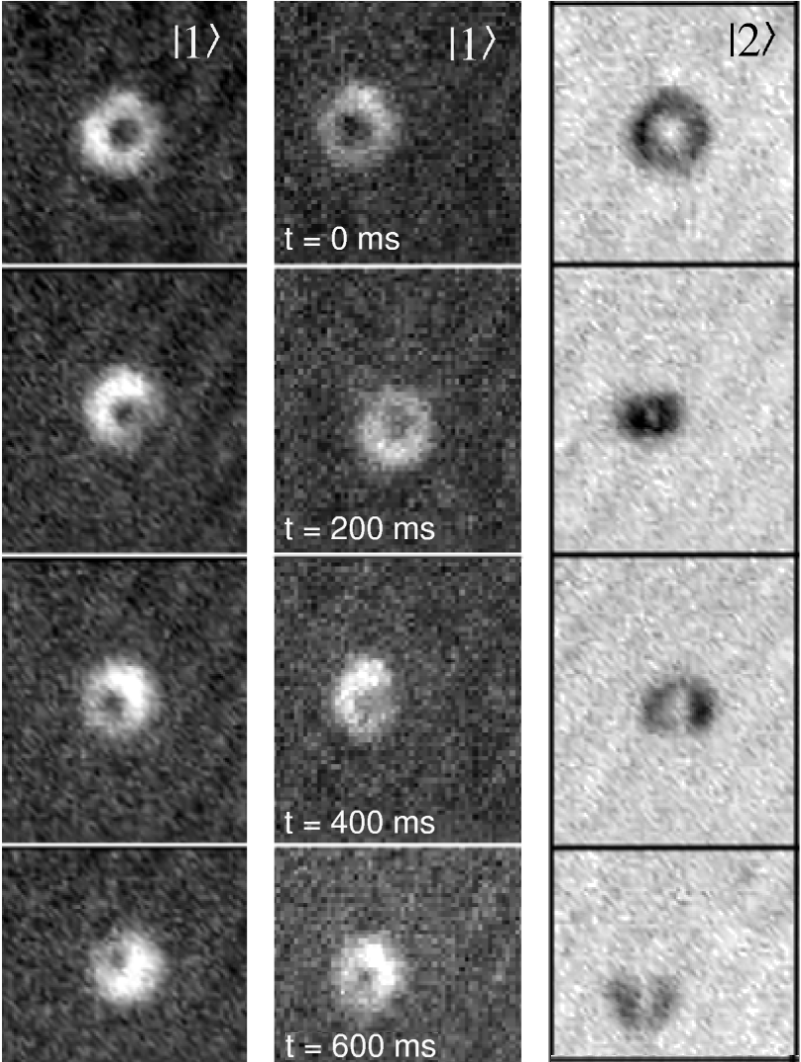
\includegraphics[width=0.5\textwidth]
    {gfx/ch-introduction/first_quantum_vortex.png}
    \caption[Experimental images of a quantum vortex in an atomic BEC]
    {\label{fig: first-vortex}Text.}
\end{figure}
Further theoretical work generalised this idea by allowing the amplitude of the
rotating laser to spatially vary instead of being confined to a
point~\cite{Ruostekoski2000}.

Due to the interactions between atoms, spinor BEC systems can energetically
favour regimes with maximal spin or minimal spin.
In a spin-1 system, these two regimes are denoted as ferromagnetic (FM) and
polar, respectively.
In each of these regimes, a variety of vortices can arise due to the differing
symmetries that are broken by the atomic interactions.
Numerous numerical works have investigated the energetic stability of singular
vortices within the FM and polar regimes, in addition to non-singular vortices
arising the FM regime.


\section{Outline of the thesis}
